\chapter{Implementation} \label{sec:implementation}
This chapter describes the implemented prototype following the architecture outlined in the above chapter (see Chapter~\ref{chapter:design}).

\section{Data Pipeline}
The knowledge base is prepared by an ingestion script \texttt{data\_pipeline/build.py}. On each run, the script loads configuration, initializes the embedding model, vector database, program store, program loader, and document loader, then builds the retrieval indexes from the robot programs and documentation data.

Keeping this workflow offline avoids performing data transformation, chunking, and embedding generation at query time. At the time of writing, the corpus consists of 8 robot programs with corresponding metadata files and 22 PDF documents, producing 8 metadata program descriptions, 126 program code chunks, and 2612 documentation chunks.

\subsection{Program Processing}
Robot programs (\texttt{.urpx} files) are loaded together with the associated \texttt{meta.json} files. Program ingestion produces two text representations: one based on the metadata and one based on the program code.

The first representation is a metadata summary. The outer loading loop iterates over all program directories, opens each \texttt{meta.json} file, and calls a helper that synthesizes exactly one \texttt{ProgramChunk} for that program (see Code~\ref{listing:implementation:program_metadata_loop}).

\begin{listing}[H]
	\begin{minted}[fontsize=\small, breaklines]{python}
programs = []
for program_dir in program_dirs:
    meta_file = program_dir / "meta.json"
    with open(meta_file, "r", encoding="utf-8") as f:
        metadata = json.load(f)

    programs.append(self._synthesize_program(program_dir.name, metadata))
	\end{minted}
	\caption{Load each program's metadata file and create one metadata chunk per program.}
	\label{listing:implementation:program_metadata_loop}
\end{listing}

% \begin{listing}[H]
% 	\begin{minted}[fontsize=\small, breaklines]{python}
% def _synthesize_program(self, program_dir: str, metadata: Dict[str, Any]) -> ProgramChunk:
% 	program_name = metadata.get("name", program_dir)
% 	robot_type = metadata.get("robotType", "Unknown")
% 	application_type = metadata.get("applicationType", "General")
% 	gripper_types = metadata.get("gripperType", [])
% 	object_type = metadata.get("objectType", [])
% 	actions = metadata.get("actions", [])
% 	data_available = metadata.get("dataAvailable", "")
% 	components = metadata.get("components", [])
%
% 	gripper_text = ", ".join(gripper_types) if gripper_types else "not specified"
% 	object_text = ", ".join(object_type) if object_type else "not specified"
% 	action_text = ", ".join(actions) if actions else "not specified"
% 	component_text = " | ".join(components) if components else "not specified"
%
% 	chunk_text = (
% 		f"Program: {program_name}. "
% 		f"Robot type: {robot_type}. "
% 		f"Application: {application_type}. "
% 		f"Gripper: {gripper_text}. "
% 		f"Object type: {object_text}. "
% 		f"Actions: {action_text}. "
% 		f"Components: {component_text}. "
% 		f"Data available: {data_available}."
% 	)
%
% 	return ProgramChunk(
% 		program_id=program_dir,
% 		program_name=program_name,
% 		chunk_text=chunk_text,
% 		metadata=metadata,
% 	)
% 	\end{minted}
% 	\caption{Helper used to synthesize the metadata summary text stored in each \texttt{ProgramChunk}.}
% 	\label{listing:implementation:program_metadata_chunk}
% \end{listing}

After the metadata file is loaded, \texttt{\_synthesize\_program(...)} extracts the program name, robot type, application type, gripper type, object type, actions, components, and data-availability field. Missing values are filled with defaults. List-valued attributes are converted into readable strings before the helper concatenates them into one natural-language sentence stored as the \texttt{chunk\_text} of the resulting \texttt{ProgramChunk} datatype. The original metadata is retained alongside it for later reference. This approach allows retrieval to operate on a natural-language summary while still preserving access to the structured metadata when needed.

Code~\ref{listing:implementation:program_metadata_example} shows an example of that synthesized text for one of the indexed programs.

\begin{listing}[H]
	\begin{minted}[fontsize=\small, breaklines]{text}
Program: Program2. Robot type: UR5. Application: Pick and Place. Gripper: 2FG7. Object type: Cube. Actions: moveJ, moveJ, release, moveL, grip, moveL, moveJ, moveL, release, moveL, moveJ. Components: UR5 | Gripper 2FG7. Data available: Robot Operational Data | Event Data.
	\end{minted}
	\caption{Example of a metadata chunk.}
	\label{listing:implementation:program_metadata_example}
\end{listing}

The second representation targets code-level retrieval and may produce multiple chunks per program. Each \texttt{.urpx} file is converted to JSON and traversed recursively by \texttt{\_collect\_nodes(...)} to locate program behavior nodes (actions). For each node, \texttt{\_extract\_action\_name(...)} tries to extract an action from parameters such as \texttt{moveType} or \texttt{action}. When an action is available, a program code chunk of type \texttt{ProgramCodeChunk} containing a natural-language summary (\texttt{chunk\_text}) and the JSON code snippet (\texttt{snippet\_text}) is created. Additional fields such as identifiers, line numbers, metadata, and chunk index are also attached to each chunk for later reference.

Code~\ref{listing:implementation:program_code_chunk} shows the code-level chunk construction.

\begin{listing}[H]
	\begin{minted}[fontsize=\small, breaklines]{python}
node_entries = []
self._collect_nodes(
	node=data.get("program", {}).get("programContent", {}),
	path="program.programContent",
	output=node_entries,
)

action_entries = []
for entry in node_entries:
	action_name = self._extract_action_name(entry)
	if action_name:
		entry["action_name"] = action_name
		action_entries.append(entry)

chunks = []
for idx, entry in enumerate(action_entries):
	chunks.append(
		ProgramCodeChunk(
			# program_id, program_name, start_line/end_line,
			# section_name, and metadata are also stored
			chunk_text=self._build_action_summary(
				program_name, entry, action_entries, idx
			),
			snippet_text=self._build_readable_snippet(entry),
		)
	)
	\end{minted}
	\caption{Program code chunk construction.}
	\label{listing:implementation:program_code_chunk}
\end{listing}

Code~\ref{listing:implementation:program_code_chunk_example} shows an example of the natural-language summary for one of the action nodes in the indexed programs.

\begin{listing}[H]
	\begin{minted}[fontsize=\small, breaklines]{text}
Program Program5 action snippet. Action: moveL; Node type: ur-move-to; Label: Point_3 | 30 % | 9 %; moveType: moveL; variable: Point_3; Previous actions: release; Next actions: moveJ.
	\end{minted}
	\caption{Example of a code-level chunk summary.}
	\label{listing:implementation:program_code_chunk_example}
\end{listing}

\subsection{Documentation Processing}
Technical documentation is processed with a dedicated PDF loader built on PyMuPDF. The extracted text is cleaned before chunking to remove common PDF artifacts such as line-break hyphenation and irregular whitespace. The cleaned text is then segmented section by section with a sentence-aware sliding window using a chunk size of 300 tokens and an overlap of 48 tokens.

Within each section, the loader first fills a chunk with as many complete sentences as fit within the target window. It then steps backward by the configured overlap so that neighboring chunks share some context. Very small trailing chunks are merged into adjacent chunks to reduce underspecified retrieval results near boundaries. Each final documentation chunk retains its document name, page number, and chunk index, yielding 2612 searchable chunks across the current document corpus.

The default chunk size of 300 tokens was chosen as a balance between contextual completeness and retrieval specificity. Smaller chunks more often separated short procedure descriptions, warnings, and parameter explanations that were semantically related, while much larger chunks increased the amount of irrelevant surrounding text returned with each hit. The overlap of 48 tokens was chosen to preserve continuity across chunk boundaries without introducing excessive duplication. In practice, this overlap was large enough to carry short transitions and neighboring procedural context into the next chunk, but small enough to avoid filling the index with near-duplicate passages.

The implementation does not compute exact token counts with the embedding model tokenizer. Instead, it uses a lightweight approximation of roughly four characters per token when translating the configured token budget into chunk-size and overlap limits. The main advantage is simplicity and performance: the chunker remains fast and independent of a model-specific tokenizer, which was useful during repeated local indexing runs. The disadvantage is reduced precision, since actual token counts vary with formatting, symbols, and vocabulary. As a result, some chunks will be somewhat shorter or longer than the target. This is also relevant with respect to the embedding model itself, because an embedding backend has a finite input window. The current implementation does not enforce a hard model-specific maximum token count, so the conservative 300 tokens with 48 token overlap also serves as a safety margin against input-limit issues, although the embedding models used have a large enough window that this was not a problem.

\subsection{Embedding and Indexing}
Embedding is handled through an \texttt{EmbeddingModel} abstraction. The wrapper reads the model name, base URL, request timeout, batch size, and embedding dimension from the data-pipeline configuration file and uses Ollama through \texttt{OllamaEmbeddings}. Its \texttt{embed()} method accepts either one string or a list of strings. For batch inputs, it slices the texts into batches of 64, calls the embedding backend for each batch, and returns a NumPy array with one vector per text. For a single query string, it returns one vector of length \texttt{embedding\_dimension}. The Qdrant vector database reads the same \texttt{embedding\_dimension} setting from config, so the embedding layer and the vector database share a single source of truth.

During early development, a smaller embedding model was used because it supported faster local indexing runs and quicker iteration on the retrieval pipeline. In the final configuration, this was replaced with \texttt{qwen3-embedding:8b}. The larger model increased indexing time, but it also improved retrieval quality.

Ingestion is implemented in \texttt{data\_pipeline/build.py}. The script initializes the embedding model, vector store, program store, and loaders, loads the three corpora, and then ingests each corpus into separate collections. For each corpus, it extracts the \texttt{chunk\_text} field, calls \texttt{embed()}, creates the Qdrant collection, and upserts one point per chunk. In Qdrant, a point is one stored vector record consisting of an id, the embedding vector, and a payload dictionary with metadata fields. The three collections are \texttt{robot\_programs} for metadata, \texttt{robot\_program\_code} for code snippets, and \texttt{documentation} for documentation.

To search a collection, the \texttt{VectorStore.search(collection\_name, query\_embedding, limit)} method is exposed. The method accepts the collection name, the query embedding vector, and the number of results to return. It then calls \texttt{query\_points(...)} on the Qdrant client, which performs a cosine similarity search and returns the top hits with their payloads and scores.


\section{Backend}
The backend is implemented as a FastAPI application with an orchestration layer. At startup, the service constructs an \texttt{Orchestrator} instance. The \texttt{Orchestrator} owns the embedding model interface, vector store connection, language model client, retrieval tools, and conversation memory.

It exposes an \texttt{invoke(...)} method that accepts a user query and optional program context. The method performs the agentic orchestration loop and then synthesizes a final response based the user query, tool-use, conversation history, and program context.

In the current implementation, both the agentic orchestration loop and the final response synthesis use the same language model, \texttt{qwen3.5:2b}.

\subsection{Agentic Loop}
The agentic functionality of the orchestrator is implemented in the \texttt{\_agentic\_loop(...)} method. Using the LangChain tool interface, the orchestrator defines three retrieval tools that the agent can call to search the program-metadata, program-code, and documentation collections. The agent is prompted to decide which tools to call and when to stop retrieving, allowing it to adaptively gather information based on the user query and the results obtained so far.

The retrieval process is implemented as an agentic loop with a fixed maximum of five steps. For each user query, the helper \texttt{\_assemble\_agent\_messages(...)} assembles the initial message list by combining the system prompt, the current query, optional program context, and conversation history. This list consists of LangChain message objects. In the current implementation, the initial entries are a \texttt{SystemMessage} containing the system prompt and \texttt{HumanMessage} objects containing the user query and additional user provided context. During the loop, the agent's reply message is appended to the same list, and each executed retrieval tool appends a \texttt{ToolMessage} containing the returned JSON payload. The agent can then stop immediately or invoke one or more retrieval tools, depending on whether the query can be answered from the current message state. After each tool call, the returned tool result is appended to the same message state and the model decides whether additional retrieval is still necessary. The five-step limit prevents the retrieval phase from continuing indefinitely in case no relevant results are returned from the tool calls.

Code~\ref{listing:implementation:agentic_loop} shows the agentic loop. The key detail is that the agent repeatedly receives the updated message state, including prior tool outputs, and can therefore stop as soon as sufficient evidence has been gathered.

\begin{listing}[H]
	\begin{minted}[fontsize=\small, breaklines]{python}
	messages = self._assemble_agent_messages(...)
	max_steps = 5

	for step_num in range(1, max_steps + 1):
		response = self.agent_llm.invoke(messages)
		messages.append(response)

		tool_calls = getattr(response, "tool_calls", []) or []
		if not tool_calls:
			sources = collect_sources_from_tool_messages(messages)
			return sources, False

		for tool_call in tool_calls:
			messages.append(self._dispatch_tool_call(tool_call, step_num, ...))

	sources = collect_sources_from_tool_messages(messages)
	return sources, True
	\end{minted}
	\caption{Agentic orchestration loop.}
	\label{listing:implementation:agentic_loop}
\end{listing}

When the agent model decides to stop (no tools called), \texttt{collect\_sources\_from\_tool\_messages(...)} filters the accumulated LangChain message list for \texttt{ToolMessage} entries produced by earlier tool calls, parses their JSON payloads, and collects the retrieved documents into one shared source list. This list is used for response synthesis regardless of which tools were called, so that the synthesis stage can reason over all retrieved information without needing to know which tool produced which result. If the loop reaches the five-step limit, the same collection process is applied to gather whatever sources were retrieved up to that point, but a boolean flag is set to indicate that retrieval may be incomplete. This allows the synthesis stage to adjust its reasoning and response generation based on whether the retrieval phase was potentially cut short by the step limit.

Code~\ref{listing:implementation:tool_registration} shows the helper that defines tools. Three retrieval tools are implemented. Each tool uses the \texttt{VectorStore.search(...)} method that performs a search over one of the three vector collections. The tools are given descriptive names such as \texttt{search\_robot\_programs}, \texttt{search\_robot\_code}, and \texttt{search\_doc\-umentation} to make their purpose clear in the system prompt. The final return statement returns the three tool objects as a list. The orchestrator later binds the list of tools to the agent model with \texttt{base\_llm.bind\_tools(...)} in the \texttt{\_bind\_agent\_llm(...)} method.

\begin{listing}[H]
	\begin{minted}[fontsize=\small, breaklines]{python}
def _define_tools(self):
	@tool("search_robot_programs")
	def search_robot_programs(query, limit=3):
		return self._search_collection(self.programs_collection, query, limit)

	@tool("search_robot_code")
	def search_robot_code(query, limit=3):
		return self._search_collection(self.program_code_collection, query, limit)

	@tool("search_documentation")
	def search_documentation(query, limit=3):
		return self._search_collection(self.documentation_collection, query, limit)

	return [search_robot_programs, search_robot_code, search_documentation]
	\end{minted}
	\caption{Tool definitions.}
	\label{listing:implementation:tool_registration}
\end{listing}

\subsubsection{Agent Prompt}
The agent behavior is shaped not only by the loop structure, but also by the system prompt produced by \texttt{get\_agentic\_system\_prompt()} in \texttt{backend/llm/prompts.py}. This prompt is inserted as the first \texttt{System\-Message} in the agent message list and frames the model as a retrieval controller rather than as the final answer generator. That separation of roles is important: during the retrieval stage, the model is instructed to gather evidence and decide whether to continue retrieving, while response synthesis is handled later by a separate prompt. The full prompt is shown in Code~\ref{listing:appendix:agent_prompt} in Appendix~\ref{appendix:implementation-prompts}.

The agent system prompt combines several prompt-engineering techniques. First, it uses \textit{role prompting} by assigning the model the role of an intelligent retrieval assistant for robot programs and documentation. Second, it uses \textit{clear and specific instructions}: the prompt states the model's job explicitly, lists the available tools, and defines a concrete retrieve-evaluate-decide workflow. Third, it uses \textit{constraint setting}. The prompt tells the model not to synthesize the final answer, limits the number of documents and tool calls, and instructs it to stop early when sufficient evidence has already been found. These constraints narrow the model's behavior from general dialogue generation to controlled evidence gathering.

The prompt also uses a constrained form of \textit{chain-of-thought prompting}. It does not ask the model to emit a free-form reasoning trace, but it does force a stepwise reasoning pattern: retrieve context, evaluate relevance and sufficiency, identify gaps, and then decide whether to stop or continue. In addition, the prompt uses \textit{few-shot learning} through four concrete decision scenarios. Those examples demonstrate the desired policy for different classes of questions, such as example-program search, technical-configuration questions, program-modification requests, and general-knowledge queries that should bypass retrieval entirely. The prompt further uses \textit{delimiter and structure cues} in the form of section headings, numbered workflow stages, and clearly separated STOP/CONTINUE conditions, which makes the instruction hierarchy easier for the model to follow.

Together, these prompt elements complement the code-level constraints in the orchestrator. The Python code enforces the message flow and the five-step limit, but the prompt shapes the model's actual retrieval strategy: which tool it selects first, whether it broadens the search after weak results, and when it decides that the available evidence is sufficient.


\subsection{Context Management}
Context management keeps the message state small enough that each request still has room for the current query, the system prompts, retrieved documents, optional program context from the editor, and recent conversation history. In this application, that balance matters because both retrieval and synthesis depend on having enough space for robot-program examples and documentation passages from the current turn.

The current implementation combines \textit{system-prompt preservation} with a \textit{sliding window} over recent conversation turns. The agent and synthesis prompts are inserted separately each time the message lists are assembled, so the main instructions stay stable from turn to turn. Conversation history is handled by the \texttt{ConversationMemory} component in \texttt{backend/orchestrator/memory.py}, which stores recent user and assistant messages and makes them available again for later requests. This gives the assistant short-term continuity across follow-up questions while keeping the prompt instructions fixed.

The size of the stored history is controlled by a budget derived from the size of the model context window. Of the available context window, 20\% is reserved for conversation history. This is used as a practical fixed budget for recent dialogue, so that most of the context window remains available for the current query, the system prompts, retrieved sources, and optional program context from the editor, which can be large. Message size is estimated with a simple heuristic based on character count, word count, and a small fixed overhead per message. When the stored history grows beyond that budget, the component first reduces the number of retained messages and then removes the oldest messages until the history fits again. The system keeps the most recent conversation turns and leaves room for the current-turn material that is most important for retrieval and synthesis.


\subsection{Response Synthesis}
After tool-use, the backend enters a separate synthesis stage implemented in \texttt{\_synthesize\_response(...)}. At this point, the agentic loop has already collected a list of source objects, and the synthesis stage converts those sources into one context block for the language model. For each retrieved item, the backend includes the retrieved text and its source label. For code-related results, it also includes the JSON snippet stored in the payload, so the model can use both the short embedding summary and the underlying program structure. If the user has provided program context from the editor, that content is appended as an additional context block. Recent conversation history is included separately, and a retrieval-status message indicates whether retrieval completed normally or whether the five-step limit was reached. The final answer is therefore generated from four main inputs: the user query, the retrieved sources, optional program context, and recent conversation history.

The synthesis prompt is defined in \texttt{get\_synthesis\_prompt\_template()} in \texttt{backend/llm/prompts.py}. The full prompt is shown in Code~\ref{listing:appendix:synthesis_prompt} in Appendix~\ref{appendix:implementation-prompts}. Unlike the agent stage, this prompt is implemented as a chat prompt with two parts: a \texttt{SystemMessage} that defines the stable response policy, and a \texttt{HumanMessage} that inserts the runtime information for the current turn. The system part tells the model to answer the current query first, use the provided context, treat conversation history as secondary context, acknowledge missing information, and respond in Markdown only. The human part provides the retrieval-status text, the current user query, the primary context assembled from retrieved sources and program context, and the secondary context assembled from recent conversation history.

The synthesis prompt uses several prompt-engineering techniques. It applies \textit{role prompting} by framing the model as a helpful assistant for UR robot programming and technical questions. It uses \textit{clear and specific instructions} by stating exactly which input should be prioritized and how the answer should be grounded in the supplied context. It uses \textit{constraint setting} by instructing the model not to append a separate citations section, to acknowledge uncertainty explicitly, and to state when the available evidence is insufficient. It also uses \textit{output-format specification} through explicit Markdown rules for headings, lists, short paragraphs, and a dedicated limitations section when information is missing or uncertain. In addition, the prompt establishes a clear hierarchy between inputs: the current query is the primary signal, retrieved documents and program context are the primary evidence, and conversation history is only secondary context for continuity.

This design separates evidence gathering from answer generation. The retrieval stage is responsible for deciding what information to collect, while the synthesis stage is responsible for turning the collected evidence into a final user-facing response. In practice, this keeps the response model focused on explanation and answer construction rather than on tool choice, and it ensures that program snippets, documentation passages, user-provided editor context, and recent dialogue are all combined in a single structured prompt before generation.


\subsection{REST API}
The REST API is the connection between the browser frontend and the Python backend. A REST API is a set of URL endpoints that a client can call with standard HTTP methods. In this system, \texttt{GET} is used to fetch stored data, while \texttt{POST} is used to send a query or trigger backend work. The API has two main purposes: it gives the frontend access to stored robot-program artifacts, and it gives the frontend a way to send search requests and assistant queries to the orchestration layer.

The service is implemented with FastAPI in \texttt{backend/main.py} and \texttt{backend/api/routes.py}. FastAPI maps each endpoint to a Python function. At startup, the application creates one \texttt{Orchestrator} instance inside FastAPI's lifespan hook and stores it in the application state, so the route handlers can reuse the same backend services. The application also enables a small CORS configuration. CORS is a browser security rule that decides which web pages are allowed to call a backend service. Here it allows the local React frontend, running on \texttt{localhost}, to access the backend during development.

Request and response formats are defined with Pydantic models. Pydantic is a Python library that checks data types and converts incoming JSON into structured Python objects. \texttt{ChatRequest} contains the user message and optional program context from the editor. \texttt{ChatResponse} packages the final answer together with the returned sources, routing metadata, and a session identifier. The search route uses its own \texttt{SearchRequest} and \texttt{SearchResponse} models.

The API supports the main frontend workflow with a small set of endpoints. \texttt{POST /api/search} is used by the search page. It embeds the query, searches the \texttt{robot\_programs} vector collection, and returns ranked matches with metadata. \verb|GET /api/programs/{program_id}/json| loads the selected program in JSON form for the editor, and \verb|GET /api/programs/{program_id}/download| returns the \texttt{.urpx} file for export. In the current frontend, assistant interaction uses \texttt{POST /api/chat/stream}. The first version of the assistant endpoint was the synchronous \texttt{POST /api/chat} route, which returns one complete JSON response after all retrieval and synthesis steps have finished. Because this interaction is slow, the later \texttt{POST /api/chat/stream} route extends the same orchestration flow with progress updates. It calls \texttt{orchestrator.invoke(...)} in a background thread, stores progress messages in a queue, and sends them back to the browser as Server-Sent Events. Server-Sent Events are a simple one-way streaming format in which the server pushes messages over one open HTTP connection. The chat panel uses these streamed events to show what the assistant is working on before the final response arrives. The editor resets server-side conversation history through \texttt{POST /api/chat/clear-memory}.


\newpage
\section{Frontend}
The frontend is implemented as a single-page React application in \texttt{app/frontend}. It provides the browser interface for program search, program inspection and editing, and assistant interaction. Client-side routing is defined with \texttt{react-router} in \texttt{App.jsx}, which exposes three routes: \texttt{/} for search, \texttt{/edit} for the editor and chat interface, and \texttt{/simulate} as a placeholder for future simulation functionality.

Persistent frontend state is managed with two React context providers. \texttt{EditorContext} stores the selected program identifier, the loaded program payload, the current editor contents, the selected code range, pending program-context snippets, chat history, and the most recent search state. \texttt{ThemeContext} stores the light/dark preference and persists it in \texttt{localStorage}. This allows the loaded program, search state, and assistant conversation to remain available when the user moves between the pages.

The search page (see Figure~\ref{fig:implementation:search_tab}) is implemented in \texttt{ProgramSearch.jsx}. The page focuses on search query input, ranking, and program selection. The interface has gone through multiple iterations of result presentation. An earlier version displayed the raw semantic similarity score for each hit, but these values were interpreted as absolute quality indicators and caused confusion. In the current version, ranking is still based on the semantic score internally, while the UI emphasizes relative order and program metadata labels (robot type, application, gripper, object type, components, and action count) instead of exposing raw scores.

\begin{figure}[H]
	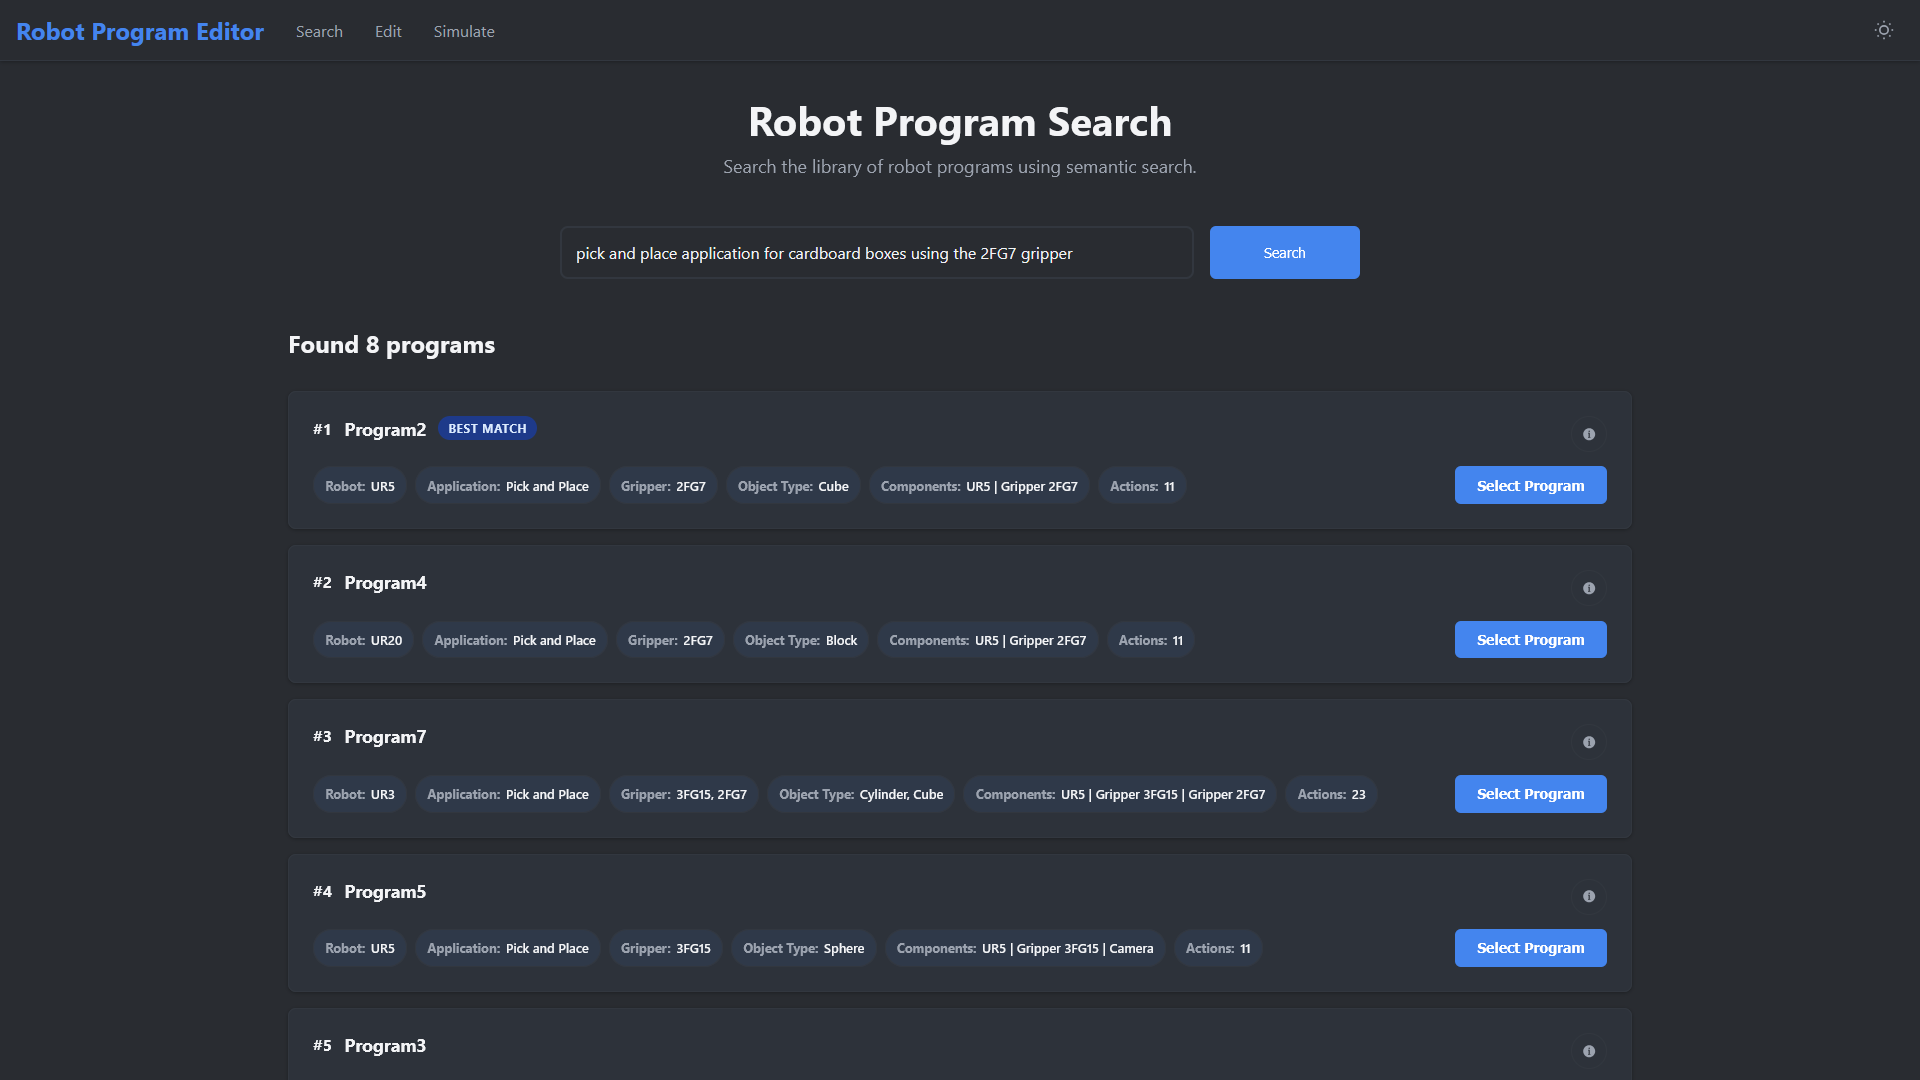
\includegraphics[width=\columnwidth]{media/search-tab.png}
	\caption{{Search page.}}
	\label{fig:implementation:search_tab}
\end{figure}

The editor tab (see Figure~\ref{fig:implementation:edit_tab}) is implemented in \texttt{Editor.jsx} as a three-panel layout using \texttt{react-resizable\-panels}. The left panel shows a generated program tree, the center panel hosts the Monaco code editor, and the right panel hosts the assistant chat. The layout is user-adjustable and persisted through the panel library so that panel widths remain consistent across revisits. This structure is designed to support assistant use directly during code inspection and editing, so program navigation, context selection, and chat interaction are available in one view. Program export is exposed through the editor menu.

\begin{figure}[H]
	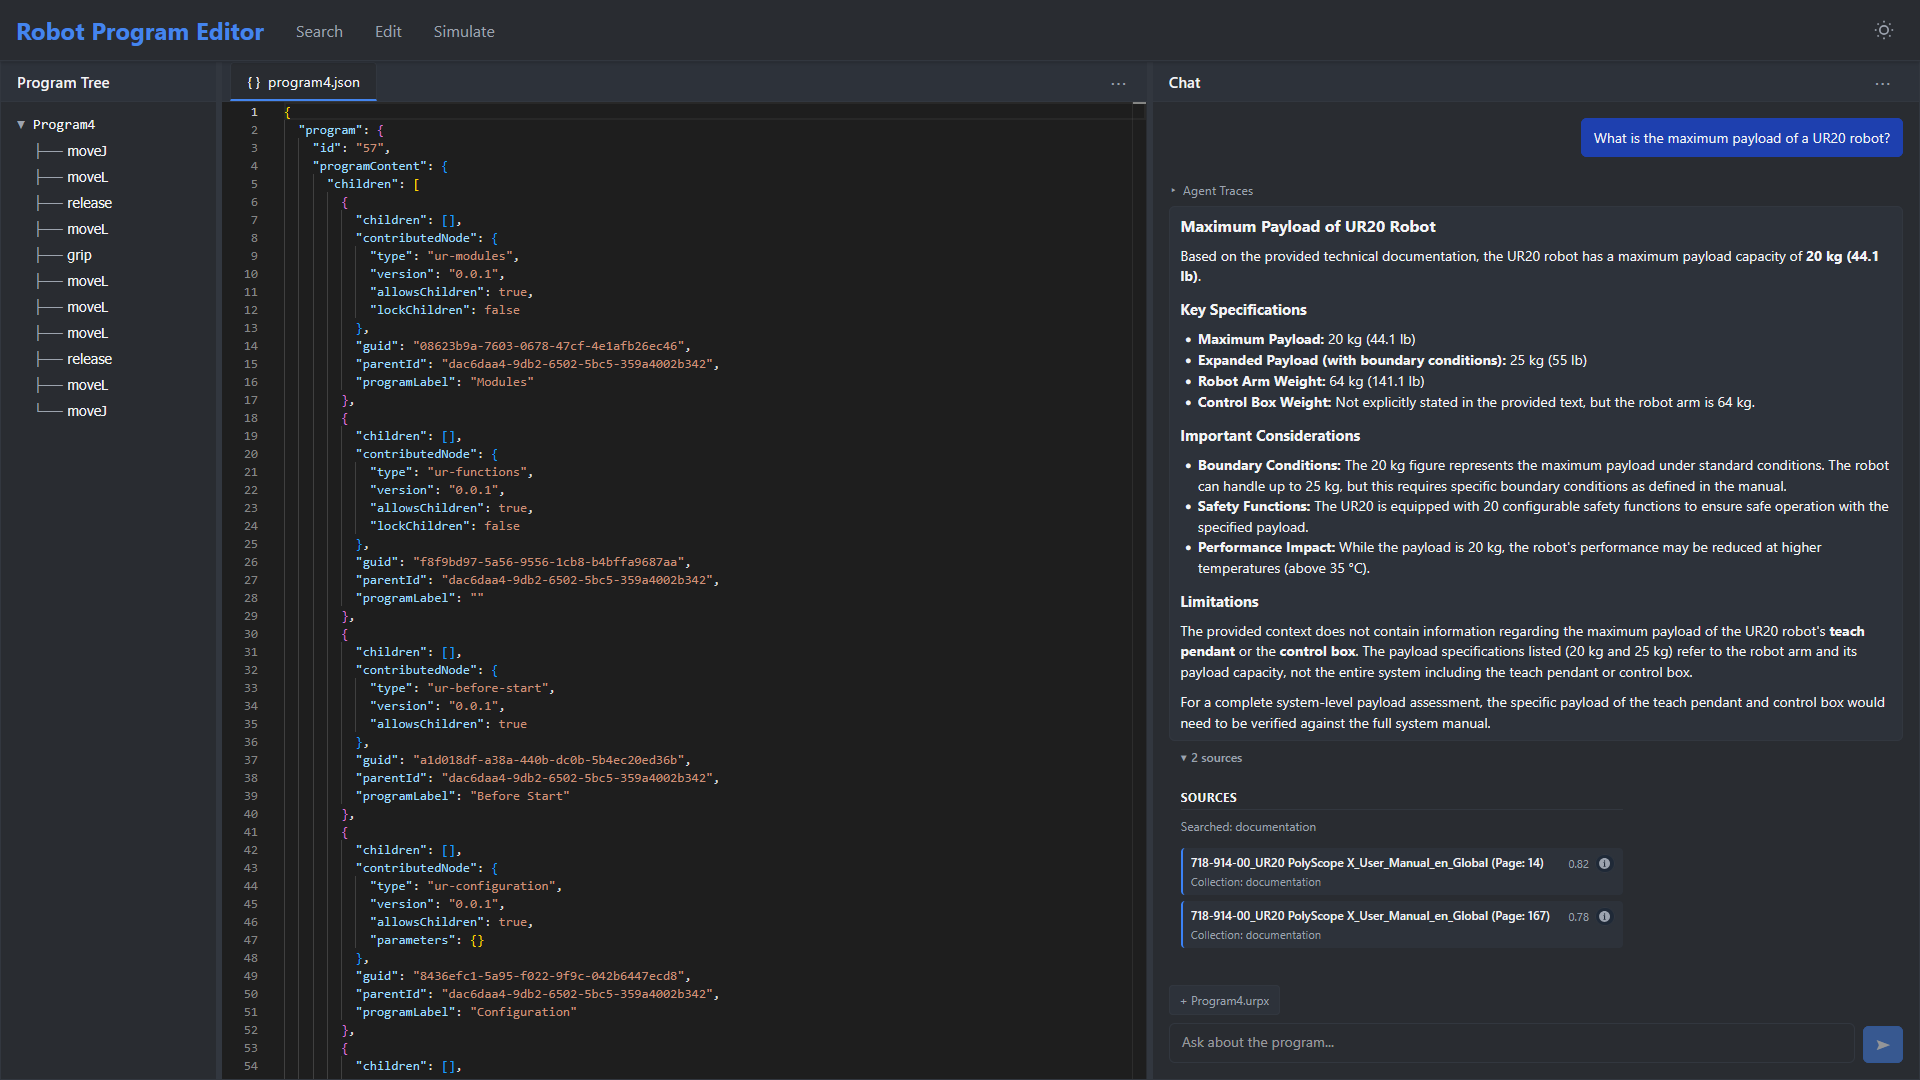
\includegraphics[width=\columnwidth]{media/edit-tab.png}
	\caption{{Edit page.}}
	\label{fig:implementation:edit_tab}
\end{figure}

The program tree is built client-side by parsing the loaded JSON and traversing the \texttt{ur-code} structure to collect action nodes. Action labels are derived from fields such as \texttt{moveType} and \texttt{action}. For each action, the frontend also resolves a corresponding line number in the editor by matching node \texttt{guid} values. Clicking a node in the program tree scrolls the code editor to the mapped location, places the cursor on that line, and centers the location in the viewport. This provides a way to navigate the program structure without needing to read through the raw code.

The chat panel, implemented in \texttt{RagChat.jsx}, supports contextual assistant interaction from within the editor workflow. The UI provides two equivalent ways to add program context: through the editor context menu and through the add-context button in the chat panel. If no code is highlighted, right-clicking in the editor and choosing the add-context action sends the entire program as context; the same full-program behavior is used when the chat-panel button is pressed without an active selection. If code is highlighted, only the highlighted line range is added. Users can attach one or more pending context snippets before asking a question, and each snippet is shown as a removable context field in the chat panel. Before transmission, \texttt{programContext.js} sanitizes the context by removing large \texttt{urscript} objects, as these are merely generated from the \texttt{.urpx} file, and so the assistant receives compact, higher-signal input.

During response generation, the interface shows live progress traces and then renders the final assistant reply as Markdown. Source details are exposed in expandable metadata blocks and hover tooltips, to provide transparency, and so users can inspect where retrieved evidence came from without leaving the editor. The chat menu also provides a clear-history action that resets both local chat state and server-side conversation memory.

